\chapter{Introduction}\label{sec:introduction}

\section{The IDSC Cubli}\label{sec:cubli}

\begin{figure}[ht]
   \centering
   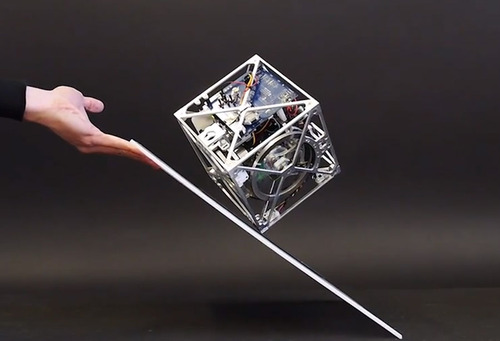
\includegraphics[width=0.75\textwidth]{img/Cubli.jpg}
   \caption{The IDSC Cubli balancing on a slanted surface.}
   \label{img:Cubli}
\end{figure}

The Cubli is a robotic cube developed at the IDSC lab in ETH Zurich, with the ability to balance on its edges and corners by using internal reaction wheels. Of relatively small size, that is dimensions of 15 x 15 x 15 cm, the robot is a proof-of-concept made possible through innovative design and engineering.

Operated by pressing buttons visible on one of cubli's faces,
\begin{figure}[ht]
   \centering
   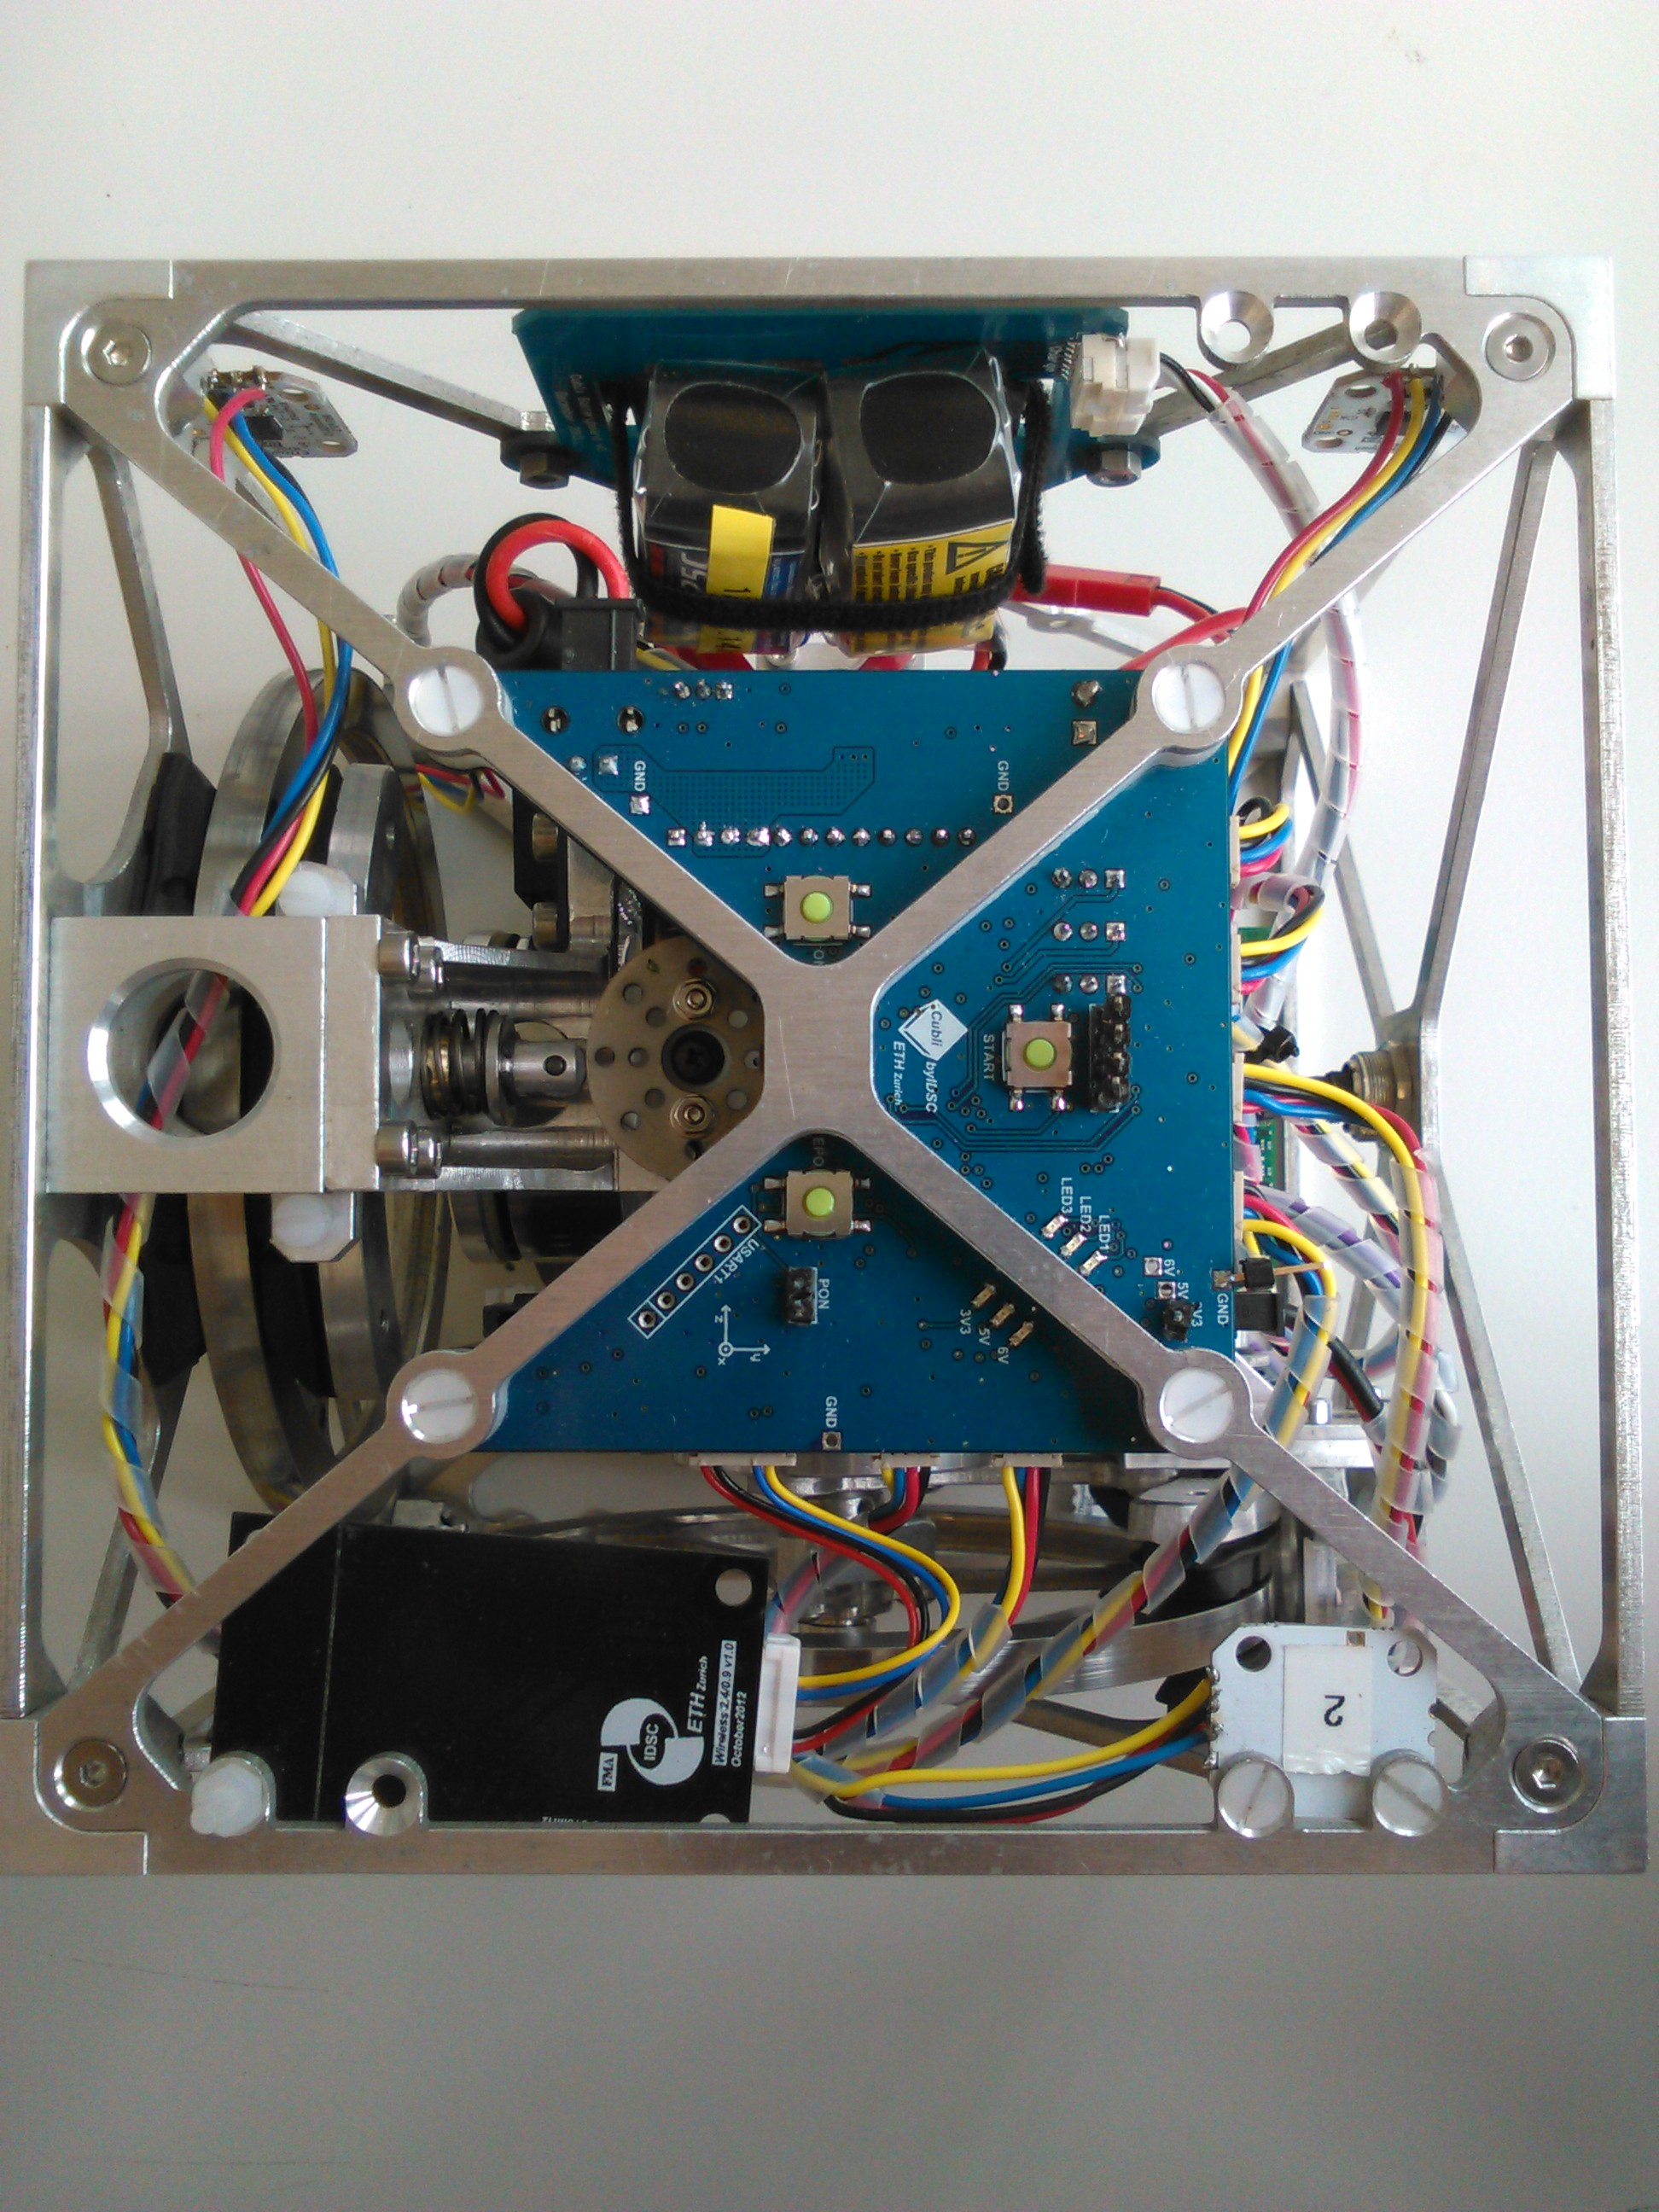
\includegraphics[width=0.75\textwidth]{img/Buttons.jpg}
   \caption{The three buttons on Cubli's controller, used to interact with cubli.}
   \label{img:Jumps}
\end{figure}
\begin{figure}[ht]
   \centering
   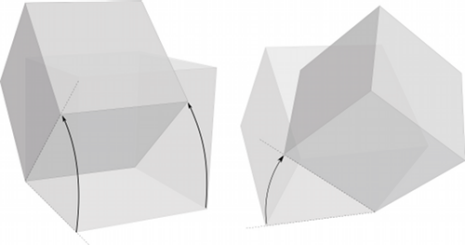
\includegraphics[width=0.75\textwidth]{img/Jumps.png}
   \caption{Illustration of Cubli's jumping abilities.}
   \label{img:Jumps}
\end{figure}